%%%%%%%%%%%%%%%%%%%%%%%%%%%%%%%%%%%%%%%%%%%%%%%%%%%%%%%%%%%%%%%%%%%%%%%%%%%%%%%
% Chapter 3 - Spatially-Targeted Photothrombotic Stroke
%%%%%%%%%%%%%%%%%%%%%%%%%%%%%%%%%%%%%%%%%%%%%%%%%%%%%%%%%%%%%%%%%%%%%%%%%%%%%%%

\chapter{Spatially-Targeted Photothrombotic Stroke} \label{Chapter_3}

Animal models of ischemic stroke are extensively used to study the mechanisms of neuronal death and recovery and to perform preliminary testing on neuroprotective interventions. While there are numerous techniques for inducing focal ischemia, the majority rely upon occlusion of the middle cerebral artery (MCA) and its branches. The MCA is the largest cerebral artery in the brain and the most common vessel involved with human ischemic events \cite{Sicard:2009ku}. The models that can most reliably reproduce the lesions and pathophysiology of human stroke (e.g. ischemic core and penumbra) offer the best experimental platforms for preclinical research.

Intraluminal MCA occlusion (MCAo) is the most widely used technique and is performed by introducing a monofilament suture into the internal carotid artery to block blood flow to the MCA \cite{Kozuimi:1986bd}. This model is capable of inducing both permanent and transient focal ischemia similar to that of human stroke and does not require craniotomy. The procedure results in large-scale infarct volumes (21-45\% of ipsilateral hemisphere) that most closely resemble malignant infarction in humans \cite{Carmichael:2005gk}. However, the majority of human strokes are much smaller in size (4.5-14\%) \cite{Carmichael:2005gk, Brott:1989bl}, making traditional MCAo a poor model for studying recovery at a similar scale. Distal MCAo produces smaller infarcts limited to the cerebral hemisphere but requires performing a craniotomy to physically access the target vessel \cite{Doyle:2014bz}. Embolic MCAo relies upon the introduction of microspheres or the induction of thrombotic clots to occlude downstream vasculature. Particle size dictates the extent and localization of the infarction, which are more variable than traditional or distal MCAo \cite{Carmichael:2005gk}. Vasoconstrictors such as Endothelin-1 (ET-1) can be injected intracerebrally in the proximity of the MCA to induce transient ischemia with a dose-dependent recovery of blood flow \cite{Sicard:2009ku}. Surgical electrocauterization or direct clipping of the MCA can also be performed to induce permanent or reversible ischemia but require craniotomy.

The photothrombosis model uses intravascular photooxidation to generate well-defined cortical lesions \cite{Watson:1985bp}. Photosensitive dyes such as rose bengal are injected intravenously and irradiated with light to produce singlet oxygen, which causes localized endothelial damage initiating platelet aggregation and thrombus formation \cite{Dietrich:1987wh}. Rose bengal has been extensively utilized as a photothrombotic agent \cite{Grome:1988bx, Parthasarathy:2010vo} and has well-characterized pharmacokinetics with fast clearance from the body \cite{Klaassen:1976kg}. A significant advantage of the photothrombotic model is the ability to stereotactically control the position and size of the infarct to target specific functional regions. However, the technique results in rapid vasogenic edema, which is thought to restrict the development of the ischemic penumbra and local reperfusion \cite{Carmichael:2005gk}.

The DMD in the imaging system offers a new method for targeting photothrombosis that allows for increased control over the stroke induction process compared to conventional techniques that only illuminate a single focal volume. Entire vessels, arbitrarily-shaped regions, or even multiple locations can be simultaneously occluded by using the DMD to pattern the irradiating light. By specifically targeting vessels, collateral photooxidative damage to the surrounding tissue can be minimized. This chapter details modifications made to the imaging system to perform DMD-targeted photothrombosis and an \textit{in vivo} demonstration of the technique in mice.



%%%%%%%%%%%%%%%%%%%%%%%%%%%%%%%%%%%%%%%%%%%%%%%%%%%%%%%%%%%%%%%%%%%%%%%%%%%%%%%
% Section 3.1 - Instrumentation Modifications
%%%%%%%%%%%%%%%%%%%%%%%%%%%%%%%%%%%%%%%%%%%%%%%%%%%%%%%%%%%%%%%%%%%%%%%%%%%%%%%
\section{Instrumentation Modifications}

The system was modified (Figure \ref{fig:systemschematic_2}) to perform photothrombotic stroke with the addition of a 532 nm laser (200 mW, AixiZ). The packaged diode laser has a 2 mm collimated output that operates at a fixed current with convection cooling. A neutral density filter (OD 1.0, NE10A-A, Thorlabs, Inc.) was used to attenuate the laser intensity by an order of magnitude down to 20 mW. A longpass dichroic beamsplitter (490 nm cutoff, DMLP490, Thorlabs, Inc.) was used to coalign the 532 nm laser with the other two lasers for coupling into the fiber optic patch cord. The green light can then be patterned by the DMD for targeted photothrombosis. \ce{pO2} measurements can be acquired simultaneously during photothrombosis induction because of the system's spectral separation, but are limited to only the stroke target region.

% Figure - System Schematic (Ver. 2)
\begin{figure}
    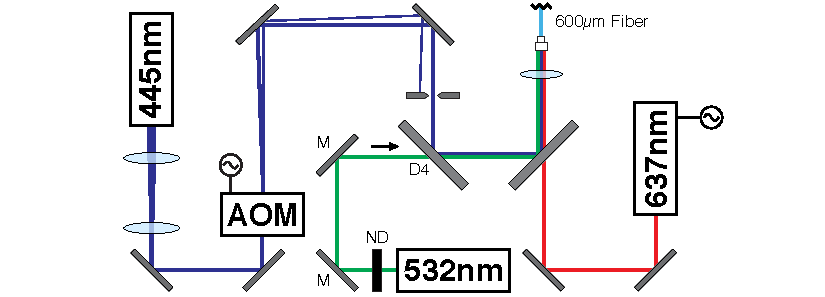
\includegraphics{figures/chapter_3/systemschematic_2.pdf}
    \caption{
        \label{fig:systemschematic_2}
        The optical system was modified with the addition of a 532 nm laser coupled into the fiber optic patch cord for DMD-targeted photothrombosis.
    }
\end{figure}



%%%%%%%%%%%%%%%%%%%%%%%%%%%%%%%%%%%%%%%%%%%%%%%%%%%%%%%%%%%%%%%%%%%%%%%%%%%%%%%
% Section 3.2 - Targeted Photothrombosis Induction
%%%%%%%%%%%%%%%%%%%%%%%%%%%%%%%%%%%%%%%%%%%%%%%%%%%%%%%%%%%%%%%%%%%%%%%%%%%%%%%
\section{Targeted Photothrombosis Induction}

Targeted photothrombosis was demonstrated \textit{in vivo} using anesthetized (1.5\% isoflurane in medical air) mice with permanent cranial window implants. Rose bengal was administered intravenously via retro-orbital injection (50 $\mu$L, 15 mg/mL) and the subject was immediately exposed to DMD-patterned green light for 5-10 minutes. Descending arterioles were the primary targets because they serve as bottlenecks in the cortical oxygen supply \cite{Nishimura:2007hk}. Target vessels were identified based on vascular orientation and \textit{a posteriori} knowledge. Because Oxyphor PtG4 has minimal absorbance of green light, \ce{pO2} measurements can be simultaneously acquired while performing photothrombosis. However, the measurements are limited to only the region being targeted for occlusion. LSCI was used to monitor clot formation within the targeted area and to control the progression of the occlusion. The speckle contrast inverse correlation times (ICT = $1/\tau_c$) were baselined against pre-stroke values to provide an estimate of the relative change in blood flow (rICT = $\tau_{c,initial}/\tau_c$).

Figure \ref{fig:photothrombosisacute} depicts the targeted photothrombotic occlusion of a descending arteriole that is likely a distal branch of the MCA. The red overlay in Figure \ref{fig:photothrombosisacute}A highlights the 0.09 mm$^2$ region irradiated with spatially-patterned green light for 420 seconds. \ce{pO2} measurements were continuously acquired from the same region at 1 Hz with 2500 decays averaged per record. The series of speckle contrast images depict the progression of the photothrombotic occlusion as the targeted vessel rapidly underwent stenosis and flow was significantly reduced. After only two minutes of exposure, the targeted vessel was indistinguishable from the surrounding parenchyma.

% Figure - Acute Photothrombosis
\begin{figure}
    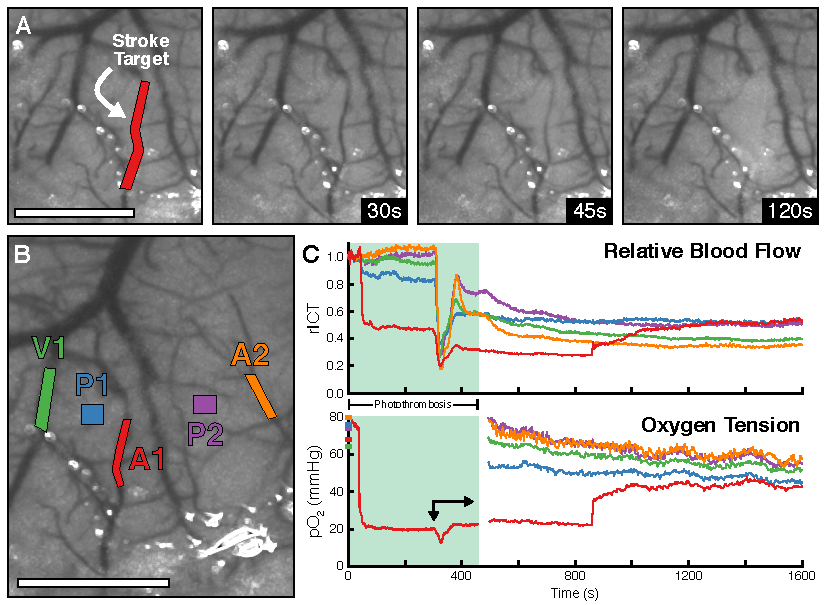
\includegraphics{figures/chapter_3/photothrombosisacute.pdf}
    \caption{
        \label{fig:photothrombosisacute}
        \textbf{(A)} Speckle contrast images depicting the occlusion of a descending arteriole using DMD-targeted photothrombosis. The red overlay indicates the 0.09 mm$^2$ region simultaneously illuminated for occlusion and \ce{pO2} measurements. \textbf{(B)} Two arterioles (A1, A2), one vein (V1), and two parenchyma regions (P1, P2) were targeted for \ce{pO2} measurements after stroke induction. \textbf{(C)} Relative blood flow and \ce{pO2} within the targeted regions during and after photothrombosis. The green-shaded section indicates irradiation of the targeted arteriole. The arrow indicates the propagation of an ischemia-induced depolarization event. (Scale bars = 1 mm).
    }
\end{figure}

% Figure - PID Propagation
\begin{figure}
    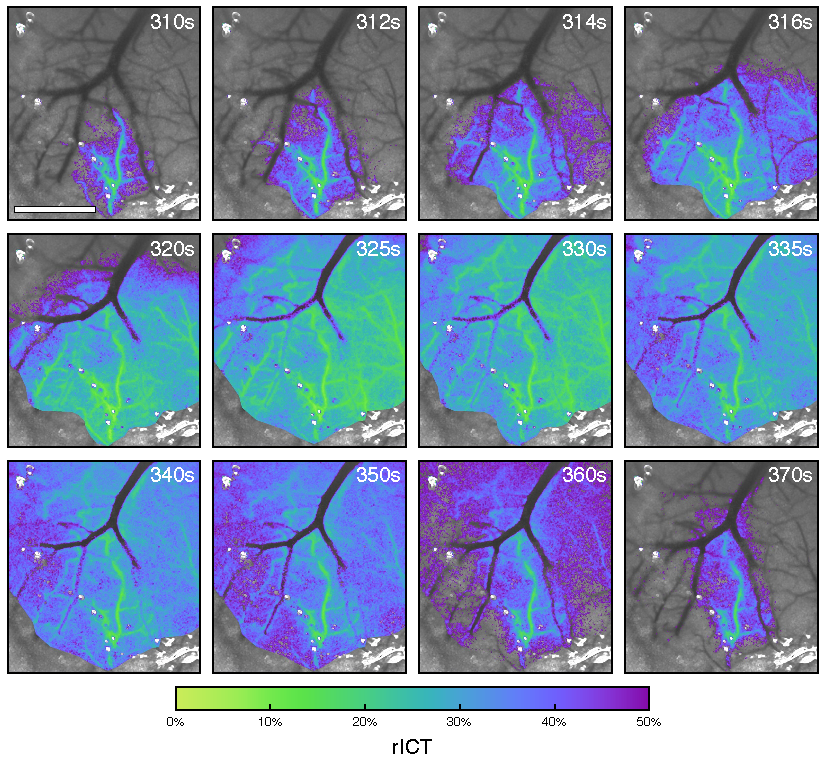
\includegraphics{figures/chapter_3/pidsequence.pdf}
    \caption{
        \label{fig:pidsequence}
        Relative flow during an ischemia-induced depolarization event that results in the expansion of the flow deficit. The depolarization has minimal effect upon the large draining vein. (Scale bar = 1 mm).
    }
\end{figure}

Figure \ref{fig:photothrombosisacute}B depicts the five regions (two arterioles, one vein, two parenchyma) targeted for dynamic relative blood flow and \ce{pO2} measurements. The first arteriole region (A1) is the same vessel targeted for photothrombotic occlusion. The resulting timecourses of relative blood flow and \ce{pO2} within each region can be seen in Figure \ref{fig:photothrombosisacute}C. By $t$ = 120 seconds, flow within the targeted arteriole had decreased to \textless50\% of baseline and \ce{pO2} had dropped from 80 mmHg to only 20 mmHg. Over the following several minutes, flow also decreased in the nearby parenchyma and venous regions (P1 and V1) and increased slightly in the distal second arteriole region (A2). The propagation of an ischemia-induced depolarization event \cite{Shin:2006dc, Dreier:2011gz} can be seen beginning at $t$ = 300 seconds, with sharp reductions in both relative blood flow and \ce{pO2}. As the depolarization subsided, flow within the targeted arteriole further decreased to \textless35\% of baseline flow while the \ce{pO2} returned to pre-depolarization levels around 20 mmHg. Flow in all other regions remained depressed immediately following the depolarization. Figure \ref{fig:pidsequence} overlays relative ICT on speckle contrast imagery to depict the spatial extent of the depolarization and the resulting increase in deficit area. This global reduction in flow following a spreading depolarization is consistent with previous studies using other stroke models \cite{Shin:2006dc, Nakamura:2010wp}.

Photothrombosis irradiation was stopped at $t$ = 420 seconds and \ce{pO2} measurements from all five ROIs were initiated. Patterns were displayed at 2 Hz with 1250 decays averaged per record. Flow and \ce{pO2} decreased over the remaining 20 minutes of the imaging session across all regions except for A1. At $t$ = 860 seconds, the targeted vessel partially reperfused, causing an abrupt increase in both relative blood flow (+6 percentage points) and \ce{pO2} (+15 mmHg). By the end of the imaging session, flow had increased within A1 to 55\% of baseline and \ce{pO2} to 42 mmHg, likely indicating further reperfusion of the vessel.



%%%%%%%%%%%%%%%%%%%%%%%%%%%%%%%%%%%%%%%%%%%%%%%%%%%%%%%%%%%%%%%%%%%%%%%%%%%%%%%
% Section 3.3 - Chronic Post-Stroke Hemodynamics
%%%%%%%%%%%%%%%%%%%%%%%%%%%%%%%%%%%%%%%%%%%%%%%%%%%%%%%%%%%%%%%%%%%%%%%%%%%%%%%
\section{Chronic Post-Stroke Hemodynamics} \label{sec:chronic_hemodynamics}

The chronic progression of the ischemic lesion was monitored for eight days following photothrombosis. The subject was anesthetized (1.5\% isoflurane in medical air) and positioned on the stereotaxic frame such that the speckle contrast imagery was aligned with previous acquisitions. Imaging sessions were kept as short as possible (\textless30 minutes) to avoid over-exposure to isoflurane. The perfusion of the occluded arteriole and broader effects on cortical flow were tracked using LSCI as shown in Figure \ref{fig:photothrombosischronic}A. Tiled \ce{pO2} maps acquired using both 445 and 637 nm excitation (Figure \ref{fig:photothrombosischronic}B-C) reveal the spatial extent of the oxygen deficit. The broad value range of the colormap masks the smaller \ce{pO2} differences between arterioles and venules. A large gradient can be seen between the occluded vessel and surrounding tissue on Days +1 and +2 despite partial reperfusion of the targeted vessel. This gradient resembles the ischemic penumbra that the photothrombotic technique rarely produces \cite{Carmichael:2005gk}. By Day +5, the targeted arteriole had fully reperfused and the hypoxic region recovered to near baseline.

% Figure - Chronic Photothrombosis
\begin{figure}
    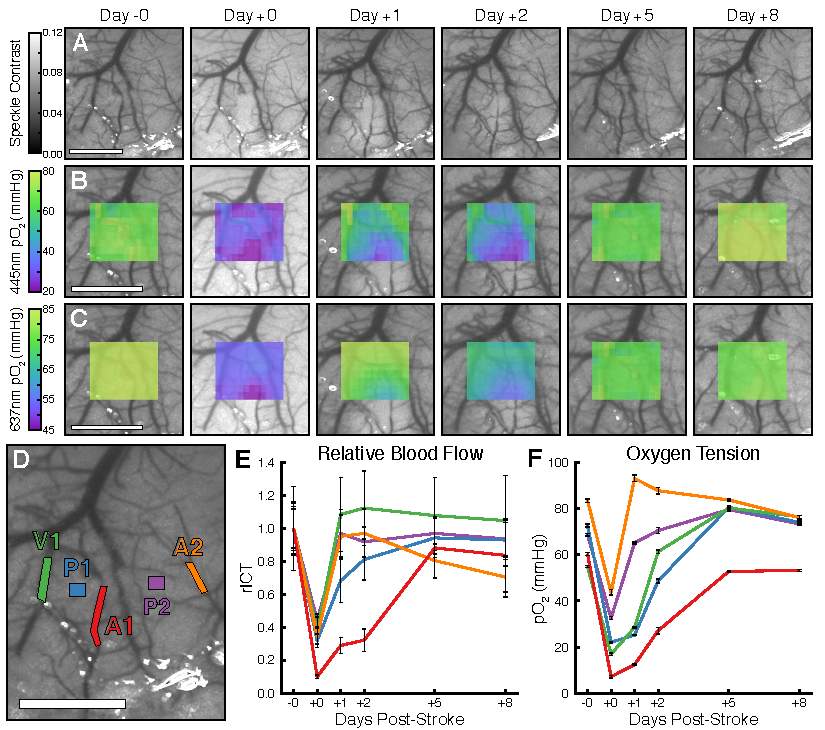
\includegraphics{figures/chapter_3/photothrombosischronic.pdf}
    \caption{
        \label{fig:photothrombosischronic}
        Progression of the ischemic lesion over eight days as imaged with \textbf{(A)} LSCI, \textbf{(B)} 445 nm tiled \ce{pO2}, and \textbf{(C)} 637 nm tiled \ce{pO2} measurements. Day -0 measurements were taken immediately prior to photothrombosis induction and Day +0 measurements were taken immediately after. \textbf{(D)} Two arterioles (A1, A2), one vein (V1), and two parenchyma regions (P1, P2) were targeted for chronic \textbf{(E)} relative blood flow and \textbf{(F)} 445 nm \ce{pO2} measurements (mean $\pm$ s.d.). The relative blood flow was baselined against Day -0 measurements. (Scale bars = 1 mm).
    }
\end{figure}

The same five regions (two arterioles, one vein, and two parenchyma) used during the acute photothrombosis measurements were also targeted for chronic relative blood flow and \ce{pO2} measurements (Figure \ref{fig:photothrombosischronic}D-F). The relative blood flow was calculated using the spatial average of the pre-stroke (Day -0) ICT measurements as the baseline. The first post-stroke measurements (Day +0) were taken immediately after the induction of photothrombosis and revealed global deficits in both blood flow and \ce{pO2}. This systemic change is likely the result of the spreading depolarization, which have previously been shown to cause global reductions in CBF using other stroke models \cite{Shin:2006dc, Nakamura:2010wp}. The blood flow and \ce{pO2} within the ROIs mirror the recovery seen in the spatially-resolved results with the vessel fully reperfusing by Day +5.

The speed of this recovery is faster than previous traditional photothrombotic inductions performed by the lab, which took 3-4 weeks to return to baseline flow levels \cite{Schrandt:2015gu}. This discrepancy can be explained by the smaller area targeted for photothrombosis (0.09 mm$^2$ vs. 0.28 mm$^2$) and the lower irradiance (\textless15 mW/mm$^2$ vs. 72 mW/mm$^2$) within the area of illumination, which resulted in a less severe ischemic lesion. Confinement of the excitation light to only within the targeted arteriole minimized collateral damage to the surrounding vasculature and parenchyma and allowed the infarct to manifest downstream of the occlusion. The lack of reperfusion is also a common critique of the photothrombotic model of stroke \cite{Carmichael:2005gk}.

%%%%%%%%%%%%%%%%%%%%%%%%%%%%%%%%%%%%%%%%%%%%%%%%%%%%%%%%%%%%%%%%%%%%%%%%%%%%%%%
\subsection{Persistence of Oxyphor PtG4 \textit{In Vivo}}

Oxyphor PtG4 is a large molecule with a molecular weight around 35 kDa. The majority of its size arises from the PEGylated hydrophobic dendrimer surrounding the PtTBP core used to increase biocompatibility. Pilot experiments with Oxyphor PdG4, an analog with a palladium core, found that it was retained in the bloodstream for hours and readily accumulated within tumors via the enhanced permeability and retention effect \cite{Esipova:2011hi}. This allowed animals to be imaged a day after being injected with 10 $\mu$M Oxyphor PdG4.

Oxyphor PtG4 persists in the bloodstream significantly longer than previously reported in literature. Strong phosphorescent decay curves have be obtained up to two weeks after an initial injection of the dye with a target blood plasma concentration of 5 $\mu$M. The mouse utilized for the targeted photothrombosis and eight days of chronic hemodynamic imaging described above was only administered a single dose of Oxyphor PtG4 on the first day of imaging. While this allows for efficient usage of a limited supply of dye, it remains unclear how and where the probe persists in the bloodstream for such an extended period of time. Phosphorescent intensity does decrease day-to-day, which means that probe does not persist indefinitely. However, if the protective dendrimer structure is being degraded, then the reliability of the lifetime measurements is a major concern and would be difficult to validate \textit{in vivo} or to replicate the appropriate testing conditions \textit{in vitro}. In order to mitigate the impact of these uncertainties, supplemental injections of Oxyphor PtG4 are administered weekly in subjects being used for chronic imaging.



%%%%%%%%%%%%%%%%%%%%%%%%%%%%%%%%%%%%%%%%%%%%%%%%%%%%%%%%%%%%%%%%%%%%%%%%%%%%%%%
% Section 3.4 - Functional Effects of Targeted Stroke
%%%%%%%%%%%%%%%%%%%%%%%%%%%%%%%%%%%%%%%%%%%%%%%%%%%%%%%%%%%%%%%%%%%%%%%%%%%%%%%
\section{Functional Effects of Targeted Stroke}

\blindtext



%%%%%%%%%%%%%%%%%%%%%%%%%%%%%%%%%%%%%%%%%%%%%%%%%%%%%%%%%%%%%%%%%%%%%%%%%%%%%%%
% Section 3.5 - Discussion
%%%%%%%%%%%%%%%%%%%%%%%%%%%%%%%%%%%%%%%%%%%%%%%%%%%%%%%%%%%%%%%%%%%%%%%%%%%%%%%
\section{Discussion}

\blindtext



%%%%%%%%%%%%%%%%%%%%%%%%%%%%%%%%%%%%%%%%%%%%%%%%%%%%%%%%%%%%%%%%%%%%%%%%%%%%%%%
% END Chapter 3
%%%%%%%%%%%%%%%%%%%%%%%%%%%%%%%%%%%%%%%%%%%%%%%%%%%%%%%%%%%%%%%%%%%%%%%%%%%%%%%
